\documentclass[11pt]{article}
\input{/Users/markwang/.preamble}
\begin{document}




\subsection*{35 Approaximation Algorithms}


\begin{defn*}
    \textbf{Performance ratio for approximation algorithms}
    \begin{enumerate}
        \item \textbf{Context} Trying to find solution to a hard optimization problem (either maximize or minimize)
        \item \textbf{Approximation ratio} An algorithm for a problem has an approximation ratio of $\rho(n)$ if for any input size $n$, the cost $C$ of the solution produced by the algorithm is within a factor of $\rho(n)$ of the cost $C^*$ of an optimal solution 
        \[
            \textsc{Max}\left( \frac{C}{C^*}, \frac{C^*}{C} \right) \leq \rho(n)
        \]
        The \textbf{range of ratio} is never less than 1. So a 1-approximation algorithm produces an optimal solution
        \item \textbf{$\rho(n)$-approximation algorithm} an algorithm achieving an approximation ratio of $rho(n)$. 
        \item \textbf{Maximization problem} $0 < C \leq C^*$, the ratio $\frac{C^*}{C}$ gives the factor by which the cost of an optimal solution is larger than the cost of the approximation algorithm
        \item \textbf{Minimization problem} $0 < C^* \leq C$, the ratio $\frac{C}{C^*}$ gives the factor by which the cost of the approximation algorithm is larger than the cost of an optimal solution 
        \item \textbf{Approximation scheme} for an optimization problem is an approximation algorithm that takes as input not only an instance of the problem, but also the value $\epsilon$ such that for any fixed $\epsilon$, the scheme is a $(1+\epsilon)$-approximation algorithm. 
        \item \textbf{Polynomial-time approximation scheme} An approximation scheme is a polynomial-time approximation scheme if for any fixed $\epsilon > 0$, the scheme runs in time polynomial in size $n$ of its input instance (the runtime can increase rapidly as $\epsilon$ decreases), i.e. $O(n^{2/\epsilon})$
        \item \textbf{Full polynomial-time approximation scheme} An algorithm is fully polynomial-time approximation scheme, if it is an approximation scheme and its running time is polynomial to both $\frac{1}{\epsilon}$ and size $n$ of input instance. $O(\frac{1}{\epsilon}n^3)$ (A constant factor decrease in $\epsilon$ comes with a corresponding constant-factor increase in running time)
    \end{enumerate}
\end{defn*}



\subsection*{35.1 Vertex Cover Problem} 

\begin{defn*}
    \textbf{Vertex Cover Problem}
    \begin{enumerate}
        \item \textbf{Vertex Cover} of an undirected graph $G = (V,E)$ is a subset $V' \subseteq V$ such that if $(u,v)\in E$, then $u\in V'$ or $v\in V'$ or both. (every edge has at least 1 vertex in the cover) That is, each vertex covers its incident edges, and a vertex cover for $G$ is a set of vertices that covers all edges in $E$.
        \item \textbf{Size of vertex cover} is the number of vertices in it 
        \item \textbf{Vertex Cover problem} the optimization problem wants to find a vertex cover of minimum size in a given graph. The decision problem wants to determine if a graph has a vertex cover of a given size $k$. 
        \[
            \textsc{Vertex-Cover} = \{\langle G, k\rangle : \text{graph $G$ has a vertex cover of size $k$} \}
        \]
        \item \textbf{Vertex Cover problem is NP-Complete}
    \end{enumerate}
\end{defn*}

\begin{defn*}
    \textbf{Proof techniques for approximation ratio} It might be puzzling to prove an exact ratio when we dont even know the size of the optimal vertex cover. Instead of trying to find the exact size of the optimal vertex cover, (for minimization problem), we rely on finding a lower bound on the size of the optimal solution. Then we relate the size of the solution to the lower bound, obtaining our approximation ratio
\end{defn*}

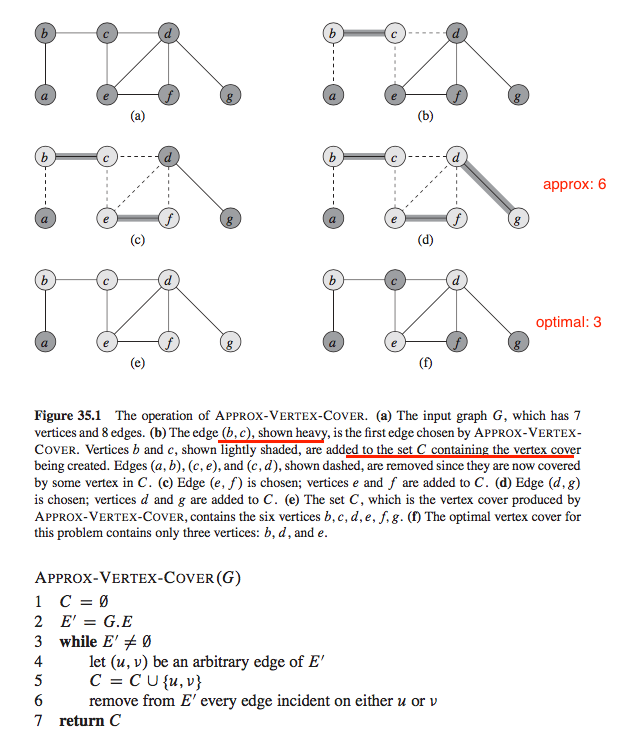
\includegraphics[width=\textwidth]{vertex_cover.png}



\begin{theorem*}
    \textsc{Approx-Vertex-Cover} is a polynomial-time 2-approximation algorithms
    \begin{proof}
        The algorithm runs in $O(V+E)$ \\
        Now we prove that \textsc{Approx-Vertex-Cover} returns a vertex cover $C$ that is at most twice the size of an optimal cover $C^*$. 
        \[
            |C| \leq 2 |C^*|
        \]
        Let $A$ denote set of edges the algorithm picked arbitrarily. Now we prove a lower bound on the optimal cover $C^*$. Note,
        \begin{enumerate}
            \item in order to cover the edges in $A$, any vertex cover, including $C^*$, must include at least one endpoint (either $u$ or $v$) for each edge $(u,v) \in A$. 
            \item No two edges in $A$ share the endpoints, since once an edge is picked, all other edges incident on its endpoints are deleted from $E'$ 
        \end{enumerate}
        Therefore, no two edges in $A$ are covered by the same vertex from $C^*$. Hence 
        \[
            |C^*| \geq |A|
        \]
        Since for any edge we pick (arbitrarily into $A$), we pick an edge for which neither of its endpoint is already in $C$, therefore we have an upper bound on the size of vertex cover returned
        \[
            |C| = 2|A|
        \]
        Therefore we have 
        \[
            |C| = 2|A| \leq 2|C^*|
        \]
    \end{proof}
\end{theorem*}


\subsection*{The Traveling-salesman problem}


\begin{defn*}
    \textbf{TSP problem} Given complete undirected graph $G= (V,E)$  with nonnegative cost $c(u,v)$ for all $(u,v)\in E$. We want to find a hamiltonian cycle (tour) of $G$ with minimum cost. Let $c(A)$ denote the total cost of edges in the subset $A\subseteq E$ 
    \[
        c(A) = \sum_{(u,v)\in A} c(u,v)
    \]
    \begin{enumerate}
        \item \textbf{Triangle Inequality} If all vertices $u,v,w\in V$, 
        \[
            c(u,v) \leq c(u,v) + c(v,w)
        \]
        Since in reality going from $u$ to $w$ is to go directly, without intermediate steps, equivalently, cutting out intermediate stop never increases the cost.
        \item \textbf{TSP with triangular inequality} is NP-complete
    \end{enumerate}
\end{defn*}


\begin{defn*}
    \textbf{Algorithm for TSP with triangular inequality}
    \begin{enumerate}
        \item Select a root 
        \item Compute a MST $T$ in $O(E\lg V)$, whose weight gives a lower bound on the length of an optimal traveling-salesman tour. 
        \item Use MST to create a tour whose cost is no more than twice that of MST's weight (as long as triangular inequality holds). Specifically order a list of vertices $H$ in the order when they are first visited in a preorder tree walk of $T$ and return the list $H$
    \end{enumerate}
    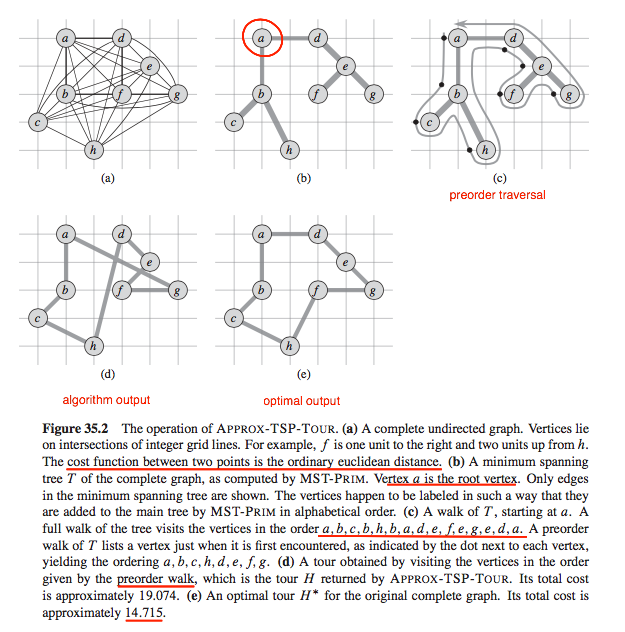
\includegraphics[width=\textwidth]{tsp.png}
\end{defn*}

\begin{theorem*}
    \textsc{Approx-TSP-Tour} is a polynomial 2-approximation algorithm for TSP problem with triangular inequality
    \begin{proof}
        Let $H^*$ denote an optimal tour of $G$ covering all vertices of $G$. We can get a MST by removing an arbitrary edge from the tour $H^*$ therefore 
        \[
            c(T)\leq c(H^*)
        \]
        Consider a full walk $W\subseteq E$ of MST $T$ when they are first visited and also whenever they are returned to after a visit to subtree, therefore $W$ traverses each edge of $T$ exactly twice, we have 
        \[
            c(W) = 2c(T) \quad \to \quad c(W)\leq 2c(H^*)
        \]
        so cost of the walk is within a factor of 2 of cost of an optimal tour. But note $W$ is generally not a tour, as it visits some vertices more than once. By triangular inequality, we can delete a visit to any vertex from $W$ and the cost would not increase. Let $H$ be the cycle corresponding to this preorder walk, with any subsequent duplicate vertices removed, yields a hamiltonian cycle (since each vertex visited exactly once). $H$ is exactly the output of the algorithm and hence 
        \[
            c(H) \leq c(W) \leq 2c(H^*)
        \]
    \end{proof}
\end{theorem*}

\begin{defn*}
    \textbf{General TSP problem} If the cost function is not restricted by triangular inequality, then we cannot find good approximate tours in polynomial time unless $P = NP$
\end{defn*}

\begin{theorem*}
    If $P\neq NP$ then for any constant $\rho \geq 1$, there is no polynomial-time approximation algorithm with approximation ratio $\rho$ for the general TSP problem
    \begin{proof}
        Proof by contradiction. Assume a $\rho \in \I$-approximation algorithm $A$ exists for general TSP. We show we can use $A$ to solve instances of \textsc{Ham-Cycle} problem in polynomial-time, which is a NPC problem and solving it in polynomial-time implies $P = NP$, arriving at a contradiction. Let $G=(V,E)$ be an instance of \textsc{Ham-Cycle}. We transform $G$ into an instance of TSP as follows. Let $G' = (V, E')$ be complete graph on $V$, that is 
        \[
            E' = \{ (u,v): u,v\in V \text{ and } u\neq v \}
        \]
        Assign integer costs 
        \[
            c(u,v)=
            \begin{cases}
                1 & \text{if } (u,v)\in E \\
                \rho|V| + 1 & \text{otherwise}\\
            \end{cases}
        \]
        This transformation can be achieved in polynomial time. Consider TSP problem $(G',c)$. If the original graph $G$ has hamiltonian cycle $H$, then $c$ assigns to each edge of $H$ a cost of 1. so $(G',c)$ contains a tour of cost $|V|$. If $G$ does not have hamiltonian cycle $H$, then any tour of $G'$ must use some edge not in $E$. But any tour using an edge not in $E$ has cost of 
        \[
            (\rho|V| + 1) + (|V| - 1) = \rho|V| + |V| > \rho |V|
        \]
        Noe edges not in $G$ is so costly, there is a gap of at least $\rho|V|$ between cost of tour that is hamiltonian in $G$ (costing $|V|$) and cost of any other tour (costing $\rho|V| + |V|$). Hence cost of tour that is not a hamiltonian cycle in $G$ is at least a factor of $\rho + 1$ greater than cost of a tour that is a hamiltonian cycle in $G$. Now apply $A$ to TSP $(G',v)$, because $A$ is guaranteed to return a tour of cost no more than $\rho$ times the cost of optimal tour, if $G$ has hamiltonian cycle, then $A$ must return it. Therefore we can use $A$ to solve hamiltonian-cycle problem in polynomial time.
    \end{proof}
\end{theorem*}

\begin{defn*}
    \textbf{Proof techniques for proving a good approximation algorithm does not exists} Suppose given NP-hard problem $X$, we can produce in polynomial time a minimization problem $Y$ such that yes instances of $X$ correspond to instances of $Y$ with value at most $k$, but no instances of $X$ correspond to instances of $Y$ with value greater than $\rho k$. THen we have shown that, unless $P=NP$, there is no polynomial-time $\rho$-approximation algorithm for $Y$
\end{defn*}




\subsection*{35.3 Set-Covering Problem}


\begin{defn*}
    \textbf{Set-Covering Problem} 
    \begin{enumerate}
        \item \textbf{Set-Covering Problem} is a generalization of vertex-cover problem and is therefore also NP-hard. An instance $(X, \mathcal{F})$ of the set-covering problem consists of a finite set $X$ and a family $\mathcal{F}$ of subsets of $X$, such that every element of $X$ belongs to at least one subset in $\mathcal{F}$
        \[
            X = \bigcup_{S\in \mathcal{F}} S
        \]
        We say that subset $S\in \mathcal{F}$ \textbf{covers} its elements. The problem is to find a minimum-size subsets $\mathcal{C} \subseteq \mathcal{F}$ whose members (subsets) cover all of $X$ 
        \[
            X = \bigcup_{S\in \mathcal{C}} S
        \]
        Any of such $\mathcal{C}$ covers $X$. The size of $\mathcal{C}$ is the number of sets it contains (not the number of elements in the set, since every subset $\mathcal{C}$ that covers $X$ must contain alll $|X|$ individual element)\\
        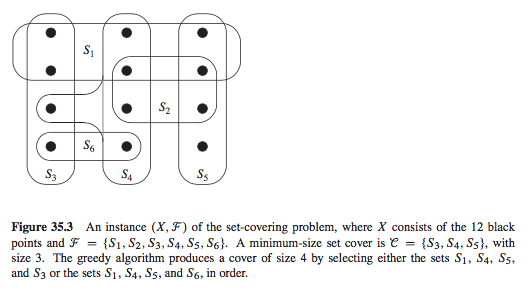
\includegraphics[width=\textwidth]{set_cover.png}
        \item \textbf{Set-Covering Decision Problem} Ask whether a covering exists with a size at most $k$, where $k$ is an additional parameter specified in the problem instanec
        \item \textbf{Harmonic number} let $d$th harmonic number be 
        \[
            H_d = \sum_{i=1}^d \frac{1}{i}
        \]
        with $H(0) = 0$
    \end{enumerate}
\end{defn*}


\begin{defn*}
    \textbf{A greedy approximation algorithm} Pick, at each stage, the set $S$ that covers the greatest number of remaining elements that are uncovered.
    \begin{enumerate}
        \item Given $(X, \mathcal{F})$
        \item Let $U = X$ be set of remaining uncovered elements
        \item Let $\mathcal{C}$ be the cover being constructed
        \item Choose a subset $S \in \mathcal{F}$ that covers as many elements as possible (i.e. maximize $|S\cap U|$)
        \item Remove $S$'s element from the remaining uncovered elements $U$
        \item Add set $S$ to $\mathcal{C}$
    \end{enumerate}  
    \begin{enumerate}
        \item \textbf{Complexity} Runtime polynomial in $|X|$ and $|\mathcal{F}|$. For loop bounded by $min(|X|, |\mathcal{F}|)$ and loop body run in $O(|X||\mathcal{F}|)$. 
    \end{enumerate}
\end{defn*}

\begin{theorem*}
    \textsc{Greedy-Set-Cover} is a polynomial-time $\rho(n)$-approximation algorithm, where $\rho(n) = H(max\{|S|: S\in \mathcal{F} \})$
\end{theorem*}


\subsection*{Randomization and Linear Programming}


\begin{defn*}
    \textbf{Randomized algorithm}
    \begin{enumerate}
        \item \textbf{Approximation ratio for random algorithm} A randomized algorithm for a problem has an approximation ratio of $\rho(n)$ if, for any input of size $n$, the \textbf{expected} cost $C$ of th solution produced by the randomized algorithm is within a factor of $\rho(n)$ of the cost $C^*$ of an optimal solution 
        \[
            max\left(\frac{C}{C^*}, \frac{C^*}{C}\right) \leq \rho(n)
        \]
        \item \textbf{Randomized $\rho(n)$-approximation algorithm} An randomized algorithm that achieves an approximation ratio of $\rho(n)$
        \item \textbf{Max-3-CNF Satisfiability} If no satisfying assignment to a boolean formula in 3-CNF form, they we which to compute how close to satisfiable it is, i.e. finding an assignment of variables that satisfies as many clauses as possible (evaluatign to 1).
    \end{enumerate}
\end{defn*}



\begin{theorem*}
    Given an instance of \textsc{Max-3-CNF} satisfiability with $n$ variables $x_1, \cdots, x_n$ and $m$ clauses, the randomized algorithm that independently sets each variable to 1 with probability $\frac{1}{2}$ and to 0 with probability $\frac{1}{2}$ is a randomized $\frac{8}{7}$-approximation algoirthm
    \begin{proof}
        Note we can assume that literals in each clause is unique and that there are no complement variables in the same clause (otherwise clause is satisfied). Set each variable $x_1, \cdots, x_n$ independently. Define indicator variable 
        \[
            Y_i = \mathbb{I}\{ \text{clause $i$ is satisfied} \}
        \]
        $Y_i$ is 1 as long as we have set at least one of the literals in the $i$th clause to 1. Since literals are unique with no complements in the same clause, the setting of 3 literals in a clause is independent. A clause is not satisfied only if all three literal evaluates to 0, i.e. $\frac{1}{8}$. So clause $i$ is satisfied with probability of $\frac{7}{8}$. Hence $\E[Y_i] = \frac{7}{8}$. Let $Y$ be number of satisfied clauses overall, we have $Y = Y_1 + Y_2 + \cdots + Y_m$
        \[
            \E[Y] = \sum_{i=1}^m \E[Y_i] = \sum_{i=1}^m \frac{7}{8} = \frac{7m}{8}
        \]
        Note $m$ is an upper bound on number of satisfied clauses, so approximation ratio is $\frac{m}{7m / 8} = \frac{8}{7}$
    \end{proof}
\end{theorem*}


\begin{defn*}
    \textbf{Linear Programming}
    \begin{enumerate}
        \item \textbf{Minimum-weight vertex-cover problem} Given an undirected graph $G = (V,E)$ in which each vertex $v\in V$ has an associated positive weigth $w(v)$. For any vertex cover $V' \subseteq V$, we define the weight of the vertex cover
        \[
            w(V') = \sum_{v\in V'} w(v)
        \]
        The goal is to find a vertex cover of minimum weight. If all weights $w(v)$ are equal to one, the problem reduces to the unweighted-vertex cover optimization problem  
        \item \textbf{0-1 integer program as a solution} Associate a variable $x(v)$ with each $v\in V$, require $x(v)$ equal either 0 or 1. Put $v$ into vertex cover if and only if $x(v) =1$. We enforce a constraint that for any edge $(u,v)$ at least one of $u$ and $v$ must be in the vertex cover as $x(u) + x(v) \geq 1$
        \begin{align*}
            \text{Minimize: } \quad & \sum_{v\in V} w(v) x(v)\\
            \text{Subjec to: } \quad & x(u) + x(v) \geq 1 \quad \text{for each } (u,v)\in E \\
            & x(v)\in \{0,1\}\quad \text{for each } v\in V\\
        \end{align*}
        If we remove constraint $x(v)\in \{0,1\}$ and replace with $0\leq x(v) \leq 1$, then we obtain a linear program, known as \textbf{linear programming relaxation} 
        \begin{align*}
            \text{Minimize: } \quad & \sum_{v\in V} w(v) x(v)\\
            \text{Subjec to: } \quad & x(u) + x(v) \geq 1 \quad \text{for each } (u,v)\in E \\
            & 0\leq x(v)\leq 1 \quad \text{for each } v\in V\\
        \end{align*}
        Note any feasible solution to 0-1 integer program is also a feasible solution to the relaxed linear program. The solution space of 0-1 ILP is a proper subset of that of the relaxed LPP, hence the value of optimal solution to the relaxed linear program is a lower bound on the value of the optimal solution to 0-1 integer program, i.e. a lower bound on optimal weight in minimum-weight vertex-cover problem. 
        \item \textbf{Algorithm}
        \begin{enumerate}
            \item initialize an empty cover $C$
            \item Compute the optimal value of $\overline{x}$ to relaxed LPP, where $0 \leq \overline{x}(v) \leq 1$
            \item For each $v\in V$ Put $v$ in vertex cover $C$ if $\overline{x}(v) \geq \frac{1}{2}$. In effect we are rounding each fractional variable in the solution to 0 or 1 in order to obtain solution to 0-1 integer program 
        \end{enumerate}
    \end{enumerate}
\end{defn*}


\begin{theorem*}
    \textsc{Approx-Min-Weight-VC} is a polynomial-time 2-approximation algorithm for the minimum-weight vertex-cover problem
    \begin{proof}
        The algorithm is polynomial, because there is a polynomial-time algorithm to solve the linear program and that the for loop runs in polynomial time. Let $C^*$ be an optimal value to the minimum-weight vertex-cover problem, let $z^*$ be the value of an optimal solution to the relaxed linear program. Since $C^*$ is a feasible solution to $z^*$, then $z^*$ must be a lower bound on $w(C^*)$
        \[
            z^* \leq w(C^*)
        \]
        Now we claim that rounding fractional values of variables $\overline{x}(v)$, we produce a set $C$ that is a vertex cover satisfying $w(C) \leq 2z^*$. 
        \begin{enumerate}
            \item To show $C$ is a vertex cover, consider any $(u,v)\in E$, we have $x(u) + x(v) \geq 1$, implying at least one of $\overline{x}(u)$ and $\overline{x}(v)$ is at least $\frac{1}{2}$. Hence at least one of $u$ and $v$ (by rounding up to 1) is in the vertex cover, so every edge is covered 
            \item Now consider the weight of cover 
            \[
                z^* = \sum_{v\in V} w(v)\overline{x}(v) \geq 
                        \sum_{v\in V: \overline{x}(v)\geq \frac{1}{2}} w(v)\overline{x}(v) \geq 
                        \sum_{v\in V: \overline{x}(v)\geq \frac{1}{2}} w(v)\frac{1}{2} = \frac{1}{2} \sum_{v\in C} w(v) = \frac{1}{2} w(C)
            \]
            so by lower bound on $C^*$ we have 
            \[
                w(C) \leq 2z^* \leq 2w(C^*)
            \]
        \end{enumerate}
    \end{proof}
\end{theorem*}


\end{document}
